%%%%%%%%%%%%%%%%%
% Methodology and Implementation %
%%%%%%%%%%%%%%%%%

This study builds on a rich body of road and graph network research by analyzing the similarities between different road networks.

\begin{figure}[h]
\centering
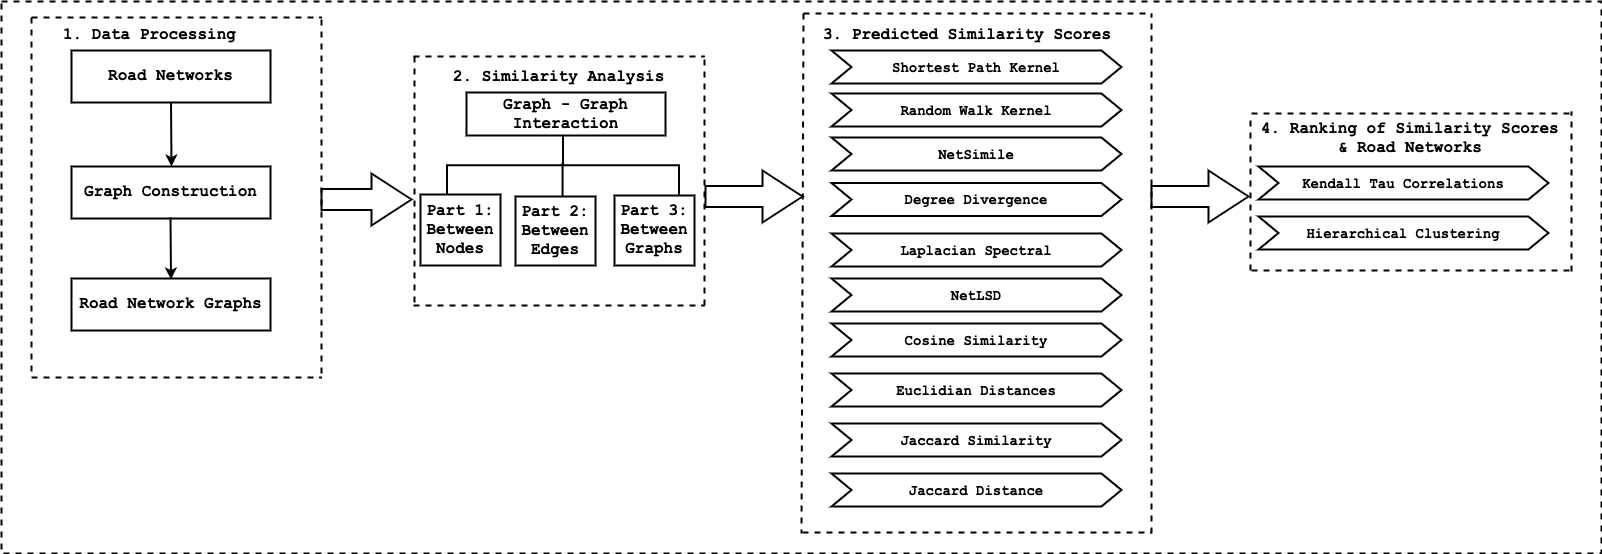
\includegraphics[width=1.25\textwidth,center]{picture/flows.png}
\caption[Methodology Workflow]{Methodology Workflow}
\label{fig:Methodology Workflow}
\end{figure}


\section{Data}
\begin{figure}[h!]
\centering
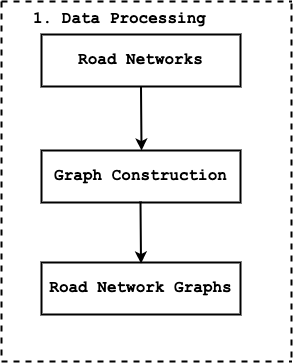
\includegraphics[width=0.35\textwidth,center]{picture/flow1.png}
\caption[Data Processing Workflow]{Data Processing Workflow}
\label{fig:Data Processing Workflow}
\end{figure}

The similarity analysis will be performed on 22 major cities worldwide, following [\cite{Louf:2014}] sampling strategy of selecting cities based on a balance of high population, regional significance, and some stratification to ensure geographical diversity within regions. The 22 sampled cities span across Africa, Asia, Australia, Europe, Middle East, North America and South America. As a result, all samples represent a diverse range of historical, cultural, developmental, and design paradigms. Of course, there is no universally accepted definition of "city" or its spatial jurisdiction throughout the world, as these differ between countries for historical and political reasons. The aim is for consistency, by trying to use each study site’s closest approximation of a “municipality” for the city limits. Once these study sites are defined, the OSMnx software [\cite{Boeing:2017}] is used to download the data and road network type for each city from OpenStreetMap. Due to its high-quality worldwide coverage, OpenStreetMap (OSM) is a collaborative online mapping platform commonly used by researchers. OpensStreetMap also provides extensive, user-contributed, open data on transport networks. OpenStreetMap’s raw data contain many interstitial nodes in the middle of street segments (forming an expansion graph) to allow streets to curve through space via a series of straight-line approximations[\cite{Boeing:2018}]. OSMnx automatically simplifies the topology for each graph to retain nodes only at intersections and dead-ends, while retaining for each edge their true spatial geometry. This provides accurate intersection counts and edge length measures for comparison between  networks with planar and nonplanar representations.[\cite{Boeing:2017}]

\section{Selected Cities}
As previously stated, this study selected 22 urban road networks from around the world, which are listed in Table \ref{tab:Selected Cities}, along with their characteristic urban form and Node and Edge size count, to determine whether road network types in different regions share any similarities. As discussed in Chapter 2, road network data sets can be classified into five basic pattern types: tree-like, grid, cul-de-sac, linear, and radial. Despite the fact that the number of 22 data sets appears to be small, this study believes that these data sets demonstrate the dependability of the study objectives and results for the following reasons. First, despite the fact that the appearance of the city varies greatly, the main pattern differences in the urban road network can be found in the shape of intersections and the density of the road network. The only thing that needs to be determined in a classification study are the characteristics of the reference network; it is not necessary to identify all of the networks one by one. Over Reliance on large-scale statistical data may make accurate identification of road network features impossible, as some features may become submerged in the massive statistical values [\cite{Han:2020}]. Furthermore, approximately 40 road network samples were chosen for on a preliminary basis for this study. Road Network samples with similar patterns and parameters were removed to clearly express the road network boundary and data distribution.
Furthermore, each sample area was limited to two square kilometers for ease of comparison. (one kilometer by one kilometer)


% Please add the following required packages to your document preamble:
% \usepackage{graphicx}
% \usepackage{lscape}
\begin{landscape}
\begin{table}[]
\resizebox{\textwidth}{!}{%
\begin{tabular}{|l|l|l|l|l|l|}
\hline
\multicolumn{1}{|c|}{\textbf{City}} &
  \multicolumn{1}{c|}{\textbf{Country}} &
  \multicolumn{1}{c|}{\textbf{Road Network Pattern (Drive)}} &
  \multicolumn{1}{c|}{\textbf{Continent}} &
  \multicolumn{1}{c|}{\textbf{Nodes}} &
  \multicolumn{1}{c|}{\textbf{Edges}} \\ \hline
Jerusalem                       & Israel      & Cul-de-sac   & Asia          & 387  & 671  \\ \hline
Amsterdam                       & Netherlands & Cul-de-Sac   & Europe        & 547  & 1049 \\ \hline
Nairobi                         & Kenya       & Radial       & Africa        & 410  & 793  \\ \hline
District of Columbia            & USA         & Grid         & North America & 461  & 1167 \\ \hline
Berlin                          & Germany     & Grid         & Europe        & 270  & 665  \\ \hline
Helsinki                        & Finland     & Grid         & Europe        & 417  & 913  \\ \hline
Toronto                         & Canada      & Grid         & North America & 325  & 827  \\ \hline
St, Petersburg, Florida         & USA         & Grid         & North America & 353  & 1069 \\ \hline
Belgrano, Buenos Aires          & Argentina   & Grid         & South America & 369  & 697  \\ \hline
Roda Island, Cairo              & Egypt       & Radial       & Africa        & 1036 & 2520 \\ \hline
Jumeirah Islands, Dubai         & UAE         & Linear       & Asia          & 93   & 198  \\ \hline
Jakarta                         & Indonesia   & Linear       & Asia          & 242  & 403  \\ \hline
Sydney                          & Australia   & Linear       & Australia     & 66   & 121  \\ \hline
Connaught Place, New Delhi      & India       & Radial       & Asia          & 391  & 853  \\ \hline
Champs-Elysees, Paris           & France      & Radial       & Europe        & 443  & 886  \\ \hline
Athens                          & Greece      & Shifted Grid & Europe        & 780  & 1405 \\ \hline
Palmanova,Friuli-Venezia Giulia & Italy       & Radial       & Europe        & 172  & 405  \\ \hline
Surulere, Lagos                 & Nigeria     & Radial       & Africa        & 280  & 629  \\ \hline
Ejecutivo, Mexico City          & Mexico      & Shifted Grid & South America & 530  & 1260 \\ \hline
Copenhagen                      & Denmark     & Shifted Grid & Europe        & 421  & 875  \\ \hline
Mumbai                          & India       & Tree         & Asia          & 363  & 826  \\ \hline
City of Westminster, London     & UK          & Tree         & Europe        & 607  & 1346 \\ \hline
\end{tabular}%
}
\caption{Selected Cities}
\label{tab:Selected Cities}
\end{table}
\end{landscape}

\begin{figure}[h!]
\centering
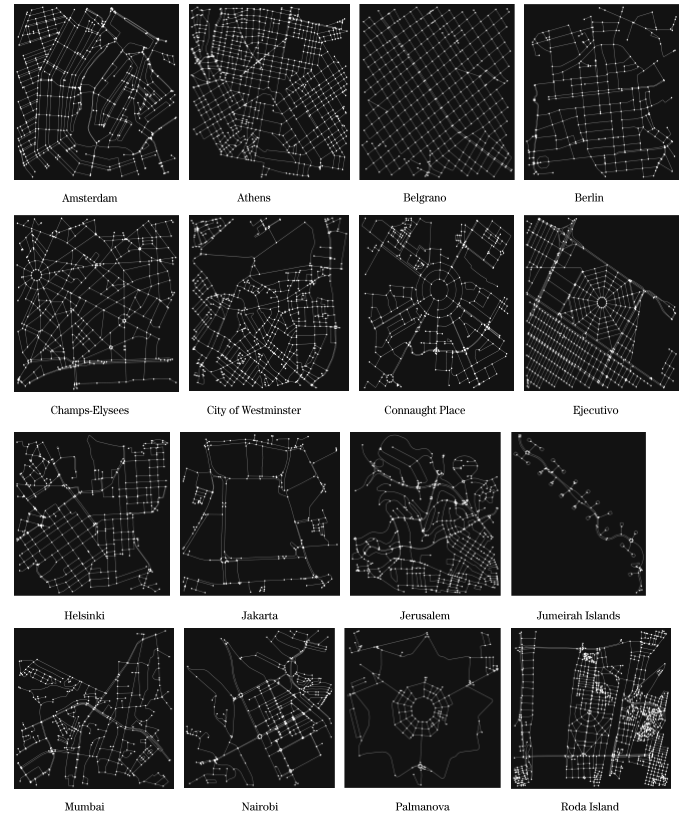
\includegraphics[width=1.0\textwidth,center]{picture/Graphs1.png}
\end{figure}

\begin{figure}[h!]
\centering
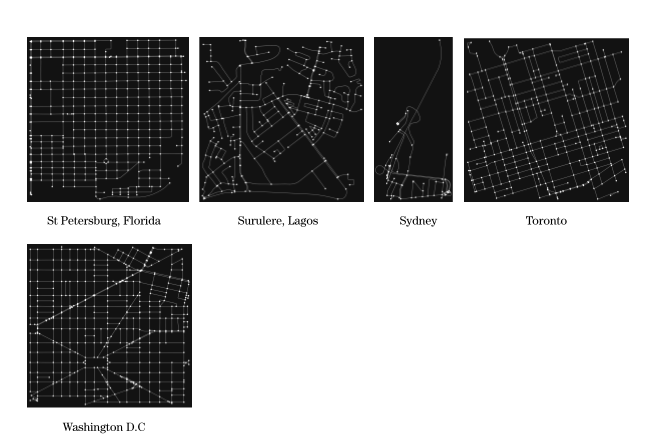
\includegraphics[width=1.0\textwidth,center]{picture/Graphs2.png}
\caption[Road Network Graphs]{Road Network Graphs}
\label{fig:roadnetworkgraphs}
\end{figure}

\section{Road Network Similarity Metrics}
All the network-similarity metrics used for this study are categorized based on two criteria. First, at what level of the network does the method operate? Second, what type of comparison does it use? 

For the first criteria, 3 levels are defined, they are micro, mezzo, and macro. As their names imply, at the micro-level, a metric extracts features at the node level;1 at the mezzo-level, the metric extracts features from communities; and at the macro-level, it extracts features from the global/network level[\cite{Soundarajan:2014}].


For the second criteria, there are 3 types: vector-based, classifier-based, and matching-based. For this study, we will be using the vector-based and classifier-based types, which are described below. 

For the Vector-based metrics, feature vectors F1 and F2 are assigned to each network G1 and G2, respectively. They define the similarity between G1 and G2 as $1-Canberra(F1, F2)$ [\cite{Richards:2010}].

For the Classifier-based metric, a fixed number of structures is first identified within each network (such as random walks, communities, or node neighborhoods). FA feature vector describing the structural properties of each of these structures (e.g., the number of edges within a node neighborhood) is calculated for each of these structures, and the feature vectors are then labeled with the name of their respective network [\cite{Soundarajan:2014}]. Cross-validation is then used afterward to determine if a Support vector machine (SVM) can accurately distinguish between the feature vectors from network G1 and the feature vectors from network G2. The test set in each round of cross-validation contains feature vectors from G1 and G2; resulting in a length-2 feature vector (respectively, F1 and F2) describing the fraction of feature vectors from that network that were classified as belonging to G1 and the fraction that were classified as belonging to G2. The similarity between G1 and G2 is defined as $1-Canberra(F1, F2)$. The SVM will be unable to distinguish between the two classes of feature vectors if G1 and G2 have very similar local structures, and F1 and F2 will be very similar. The distance between F1 and F2 will be very short, resulting in a high degree of similarity. If G1 and G2 have drastically different structures, the SVM will have a high classification accuracy but a low similarity score.

For the matching-based metric, see [\cite{Soundarajan:2014}] which goes into detail how this approach is described and can be applied. 

Table \ref{tab:Road Network Similarity Methods} categorizes all road network-similarity metrics based on the two criteria mentioned above. Each of these 10 metrics is briefly described below. Based on previous studies and research [\cite{Soundarajan:2014}], because macro-level metrics consider the entire network at once, rather than local sub-structures, it is not possible for such metrics to be classifier- or matching-based.

\begin{table}[!h]
\centering
\begin{tabular}{|p{3cm}|p{3cm}|p{3cm}|p{3cm}|}
\hline
& \textbf{Micro-Level} & \textbf{Mezzo-level} & \textbf{Macro-level} \\ \hline
\textbf{Vector-Based} & NetSimile, Euclidean Distance, Cosine Similarity  & Random Walk & Degree Divergence, NetLSD, Laplacian Spectra \\ \hline
\textbf{Classifier-Based} & Jaccard Similarity & Shortest Path Kernel, Jaccard Distance  & - \\ \hline
\end{tabular}
\caption{Road network similarity methods used in this study organized by (1) network level and (2) comparison type}
\label{tab:Road Network Similarity Methods}
\end{table}

\subsection{Shortest Path Kernel}

According to [\cite{Karsten:2005}], the shortest-path kernel decomposes graphs into shortest paths and compares pairs of shortest paths consistent with their lengths and also the labels of their endpoints. The first step of the shortest-path kernel is to transform the input graphs into shortest-paths graphs[\cite{Siglidis:2018}]. Given an input graph , a new graph  (i.e. its shortest-path graph) is created. The shortest-path graph  contains the same set of vertices as the graph from which it originates. The edge set of the former is a superset of that of the latter, since in the shortest-path graph , there exists an edge between all vertices which are connected by a walk within the original graph . To complete the transformation, labels are assigned to all the edges of the shortest-path graph . The label of each edge is set equal to the shortest distance between its endpoints within the original graph .

Given the above procedure for transforming a graph into a shortest-path graph, the shortest-path kernel is defined as follows:

Using [\cite{Karsten:2005}]  approach as illustrated in equation's 3.3.1 and 3.3.2, let Gi, Gj be two graphs and Si, Sj as their shortest-path graphs. The shortest-path kernel is then defined on Si  = (Vi, Ei) and Si = (Vj, Ej) as:

\begin{equation}
k\left(S_{i}, S_{j}\right)=\sum_{e_{i} \in E_{i}} \sum_{e_{j} \in E_{j}} k_{w a l k}^{(1)}\left(e_{i}, e_{j}\right)
\end{equation}
Source: \cite{Siglidis:2018}

where $k_{w a l k}^{(1)}\left(e_{i}, e_{j}\right)$ is a positive semidefinite kernel on edge walks of length $1 .$

The $k_{\text {walk }}^{(1)}\left(e_{i}, e_{j}\right)$ kernel in labeled graphs is designed to compare both the lengths of the shortest paths corresponding to edges $e_{i}$ and $e_{j}$, as well as the labels of their endpoint vertices.

Let $e_{i}=\left\{v_{i}, u_{i}\right\}$ and $e_{j}=\left\{v_{j}, u_{j}\right\}$. Then, $k_{\text {walk }}^{(1)}\left(e_{i}, e_{j}\right)$ is usually defined as:

\begin{equation}
\begin{aligned}
k_{\text {walk }}^{(1)}\left(e_{i}, e_{j}\right) &=k_{v}\left(\ell\left(v_{i}\right), \ell\left(v_{j}\right)\right) k_{e}\left(\ell\left(e_{i}\right), \ell\left(e_{j}\right)\right) k_{v}\left(\ell\left(u_{i}\right), \ell\left(u_{j}\right)\right) \\
&+k_{v}\left(\ell\left(v_{i}\right), \ell\left(u_{j}\right)\right) k_{e}\left(\ell\left(e_{i}\right), \ell\left(e_{j}\right)\right) k_{v}\left(\ell\left(u_{i}\right), \ell\left(v_{j}\right)\right)
\end{aligned}
\end{equation}
Source: \cite{Siglidis:2018}

$k_{v}$ is the kernel that compares vertex labels, while $k_{e}$ is the kernel that compares shortest path lengths. Vertex labels are typically compared using a dirac kernel, while shortest path lengths are compared using a dirac kernel or, less frequently, using a a brownian bridge kernel [\cite{Karsten:2005}].

In terms of runtime complexity, the shortest-path kernel is very expensive because it takes $\mathcal{O}\left(n^{4}\right)$ computation time. [\cite{Siglidis:2018}]

\subsection{Random Walk Kernel}
The random walk kernels are probably the most well-studied family of graph kernels, which quantify the similarity between two graphs based on the number of common walks in the two graphs [\cite{Kashima:2003, Gartner:2003, Mahé:2004, Karsten:2005, Vishwanathan:2010, Sugiyama:2015, Siglidis:2018}].

This family of kernels has focused primarily on counting matching walks in the two input graphs. Random walk kernels come in several variations. The $k$ step random walk kernel compares random walks in the two graphs up to length.  The geometric random walk kernel [\cite{Gartner:2003}]is the most widely used kernel in this family, comparing walks up to infinity and assigning a weight $\lambda^{k}(\lambda<1)$ to walks of length $k$ to ensure convergence of the corresponding geometric series. Following that, a formal definition of the geometric random walk kernel is defined below. 

Given two node-labeled graphs $G_{i}=\left(V_{i}, E_{i}\right)$  and $G_{j}=\left(V_{j}, E_{j}\right)$ , their direct product $\boldsymbol{G}_{\times}=\left(V_{\times}, \boldsymbol{E}_{\times}\right)$ is a graph with vertex set:

\begin{equation}
V_{\times}=\left\{\left(v_{i}, v_{j}\right): v_{i} \in V_{i} \wedge v_{j} \in V_{j} \wedge \ell\left(v_{i}\right)=\ell\left(v_{j}\right)\right\}   
\end{equation}
Source: \cite{Siglidis:2018}

and edge set:

\begin{equation}
E_{\times}=\left\{\left\{\left(v_{i}, v_{j}\right),\left(u_{i}, u_{j}\right)\right\}:\left\{v_{i}, u_{i}\right\} \in E_{i} \wedge\left\{v_{j}, u_{j}\right\} \in E_{j}\right\} 
\end{equation}
Source: \cite{Siglidis:2018}

A random walk on $G_{\times}$ is equivalent to performing a simultaneous random walk on both $G_{i}$ and $G_{j}$. As the geometric random walk kernel counts the common walks (of potentially infinite length) in the two graphs, it can therefor be defined as follows.

\subsubsection{Definition: Geometric Random Walk Kernel}

According to [\cite{Siglidis:2018}], Let $G_{i}$ and $G_{j}$ be two graphs, with $A_{\times}$denoting the adjacency matrix of their product graph $G_{\times}$ and $V_{\times}$ denoting the product graph's vertex set $G_{\times}$.

Then, the geometric random walk kernel is defined as:

\begin{equation}
K_{\times}^{\infty}\left(G_{i}, G_{j}\right)=\sum_{p, q=1}^{\left|V_{\times}\right|}\left[\sum_{l=0}^{\infty} \lambda^{l} A_{\times}^{l}\right]_{p q}=e^{T}\left(I-\lambda A_{\times}\right)^{-1} e  
\end{equation}
Source: \cite{Siglidis:2018}

where $I$ represents the identity matrix, $e$ represents the all-ones vector, and $\lambda$ is a positive, real-valued weight. Only if $\lambda<\frac{1}{\lambda_{\times}}$where $\lambda_{\times}$is the largest eigenvalue of $A_{\times}$ does the geometric random walk kernel converge.

In terms of runtime complexity, the direct computation of the geometric random walk kernel requires $\mathcal{O}\left(n^{6}\right)$ time. Because of its computational complexity, the method's applicability to real-world applications is severely limited. To address this problem, [\cite{Vishwanathan:2010}] in their work proposed four efficient methods to compute random walk graph kernels which generally reduce the computational complexity from $\mathcal{O}\left(n^{6}\right)$ to $\mathcal{O}\left(n^{3}\right)$. Other random walk kernel extensions are proposed by [\cite{Mahé:2004}], they specifically proposed a label enrichment approach that increases specificity while decreasing computational complexity in the majority of cases. To deal with the problem of "tottering," they also used a second order Markov random walk. [\cite{Sugiyama:2015}] concentrated on a different random walk kernel problem, a phenomenon known as "halting."


\subsection{Network Laplacian Spectral Descriptor (NetLSD)}
NetLSD is a permutation- and size-invariant, scale-adaptive, and efficiently computable graph representation method that allows for straightforward comparisons of large graphs.NetLSD creates a compact signature that inherits the Laplacian spectrum's formal properties, particularly its heat or wave kernel, and thus hears the shape of a graph. [\cite{Tsitsulin:2018}]

The NetLSD distance LSD between two graphs, $G$ and $G^{\prime}$, is the Frobenius norm between the heat trace signatures of the normalized Laplacians $\mathbf{L}$ and $\mathbf{L}^{\prime}$[\cite{Tsitsulin:2018}]. The heat kernel matrix is calculated as

\begin{equation}
H_{t}=e^{-t \mathbf{L}}=\sum_{j=1}^{n} e^{-t \lambda_{j}} \phi_{j} \phi_{j}^{T}
\end{equation}
Source: \cite{Tsitsulin:2018}

The amount of heat transferred from node $v_{i}$ to node $v_{j}$ at time $t$ is stored in the $i j$-th element of $H_{t}$[\cite{Tsitsulin:2018}]. The heat trace $h_{t}$ from the heat kernel matrix $H_{t}$ is defined as:

\begin{equation}
h_{t}=\operatorname{Tr}\left(H_{t}\right)=\sum_{j=1}^{n} e^{-t \lambda_{f}}  
\end{equation}
Source: \cite{Tsitsulin:2018}

The set $\left\{h_{t}\right\}_{t \geq 1}$ is the heat trace signature of graph $G$. The heat trace signatures of both $G$ and $\bar{G}^{\prime}$ are first computed and then compared using a Frobenius norm.

\begin{equation}
D_{\mathrm{LSD}}\left(G, G^{\prime}\right)=d_{\mathrm{FRO}}\left(\left\{h_{t}\right\}_{t \geq 0},\left\{h_{t}^{\prime}\right\}_{t \geq 0}\right)
\end{equation}
Source: \cite{Tsitsulin:2018}

In terms of runtime complexity, the computational complexity of LSD is $O\left(n^{3}\right)$ because of the spectral decomposition of both graphs' Laplacian matrices.

\subsection{Degree Divergence}
The degree divergence also known as the degree distribution Jensen-Shannon divergence [\cite{Lin:1991}] is the graph distance measure between the empirical degree distributions of two graphs. The descriptor $\psi_{G}$ is the empirical degree distribution encoded in the set of numbers $\left\{p_{k}(G)\right\}_{k \geq 0}:=\mathbf{p}$ given by $p_{k}(G):=n_{k}(G) /n$ for a $n$-node graph $G$, where $n_{k}(G)=\sum_{i=1}^{n} 1\left\{k_{i}=\right.$ $k\}$. $k_{i}=$ $\sum_{j=1}^{n} A_{i j}$ is the degree of node $i$ in terms of the adjacency matrix A of $G$, with $1\{-\}$ being the indicator function.  The Jensen-Shannon divergence between two such distributions [\cite{Carpi:2011}] is the degree JensenShannon divergence or DJS distance between the graphs [\cite{Tsitsulin:2018}]:

\begin{equation}
D_{\text {DJs }}\left(G, G^{\prime}\right)=H\left[\mathbf{p}_{+}\right]-\frac{1}{2}\left(H[\mathbf{p}]+H\left[\mathbf{p}^{\prime}\right]\right)
\end{equation}
Source: \cite{Tsitsulin:2018}

where $\mathbf{P}_{+}=\left\{\left(p_{k}+p_{k}^{\prime}\right) / 2\right\}_{k \geq 0}$ denotes a mixture distribution, and $H[\mathbf{p}]=-\sum_{k} p_{k} \ln p_{k}$ denotes the Shannon entropy. 

In terms of runtime complexity, the computational complexity of degree divergence is $O(n)$, which results from computing two degree distributions (which is $O(n)$ ) and then comparing them (which is $O\left(k_{+}\right)$, with $k_{+}<n$ being the maximum degree in either network)\cite{Tsitsulin:2018}.

\subsection{Laplacian Spectrum Distances}
Laplacian Spectrum distance is the graph distance measure between the Laplacian spectra of $G_1$ and ${G_2}$. The spectra of both normalized and unormalized Laplacian matrices are computed. The discrete spectra are then convolved with a kernel to generate continuous ones. Finally, a metric is used to compare these distributions. The results dictionary also keeps a 2-tuple of the underlying adjacency matrices in the key $adjacency$ $matrices$, the Laplacian matrices in $laplacian$ $matrices$, and the Laplacian eigenvalues in $eigenvalues$. If the compared networks are directed, the augmented adjacency matrices are computed and stored in $augmented$ $adjacency$ $matrices$. [\cite{Tsitsulin:2018}] goes into greater detail about calculating Laplacian Spectrum Distances.

In terms of runtime complexity, the computational complexity of laplacian spectrum distances is $O(n^{3})$, which results from the spectral decomposition of the laplacian matrices of both graphs [\cite{Tsitsulin:2018}].

\subsection{NetSimile}
NetSimile is a method for comparing two graphs, $G$ and $G^{\prime}$, based on their statistical features [\cite{Tsitsulin:2018}]. It is invariant to graph labels and can compare graphs of varying sizes [\cite{Berlingerio:2012}]. It is calculated as the Canberera distance between each graph's $7 \times 5$ feature matrix, $\mathbf{p}$ and $\mathbf{p}^{\prime}$. To construct the $\mathbf{p}$ and $\mathbf{p}^{\prime}$ feature matrices, first a $7 \times n$ matrix is constructed for each, with each column, $j$, consisting of the seven node-level quantities listed below [\cite{Tsitsulin:2018}]:

1. degree, $k_{j}=\sum_{j} A_{i j}$

2. clustering coefficient, $c_{j}=\left(A^{3}\right)_{j j} /\left(\begin{array}{c}k_{j} \\ 2\end{array}\right)$

3. average neighbor degree $k_{j}^{(n n)}=\frac{1}{k_{j}} \sum_{i} k_{i} A_{i j}$.

4. average clustering coefficient of the nodes in the ego network $c_{j}^{(e g o)}=\sum_{i} c_{i} A_{i j}$

5. number of edges within the ego network $T_{j}=$ $\sum_{l, m} A_{j l} A_{l m} A_{m j}$

6. number of outgoing edges from the ego network $O_{j}=\sum_{i} A_{i j} k_{i}-T_{j}=k_{j} k_{j}^{(n n)}-T_{j}$

7. number of neighbors of the ego network $n n_{j}^{(e g o)}=$ $\sum_{i} 1_{\left\{\exists l \in \mathcal{N}_{f}: i \sim l, i \chi_{j}\right\}}$


The node-level quantities are then summarized into $\mathbf{p}$ and $\mathbf{p}^{\prime}$, which are $7 \times 5$ signature vectors consisting of the median,mean, standard deviation, skewness, and kurtosis of each feature. NetSimile uses the Canberra distance to arrive at a final scalar distance.[\cite{Tsitsulin:2018}]

\begin{equation}
D_{\mathrm{KSE}}\left(G, G^{\prime}\right)=d\left(\mathbf{p}, \mathbf{p}^{\prime}\right)=\sum_{i=1}^{n} \frac{\left|p_{i}-p_{i}^{\prime}\right|}{\left|p_{i}\right|+\left|p_{i}^{\prime}\right|}
\end{equation}
\caption{Source: \cite{Tsitsulin:2018}}

In terms of runtime complexity, the computational complexity of NetSimile depends on two parts: features extraction and features aggregation. Because features are all locally defined, selecting a random edge and choosing an endpoint will take $O(q n)$, where $q$ is the average degree of a node [\cite{Henderson:2011}]. Hence, the overall complexity is $O(q n+n \log n)$, because the feature aggregation is $O(n \ln n)$ [\cite{Berlingerio:2012, Tsitsulin:2018}.

\subsection{Cosine Similarity}
Originally used in text mining for document comparison, the cosine similarity computes the angle between the document vectors, without taking into account their lengths. It assigns higher similarity to vectors that point roughly in the same direction.[\cite{scikit-learn}]
The cosine similarity values calculated are in the range $\mathrm[-1, 1]$ and are then converted to a similarity measure in the range $\mathrm[0, 1]$. According to literature [\cite{Han:2012}], the most prevalent ways of deriving the similarity measure are the following:

1. $s=1-d$

2. $s=\frac{1}{d}$

3. $s=\frac{1}{1+d}$ for unbounded $d$

4. $s=e^{-d^{2}}$

\subsection{Euclidean Distance}
Based on the Euclidean distance measurement approach, the euclidean based similarity  is a normalized euclidean similarity measure that calculates the shortest distance between 2 points irrespective of their dimensions.  The calculated distance $d$ converted to a similarity measure $s$ in the range $\mathrm[0, 1]$.[\cite{scikit-learn}]

\subsection{Jaccard Similarity}
Originally developed by Paul Jaccard [\cite{Jaccard:1901}], the Jaccard similarity also known as the Jaccard index or Jaccard similarity coefficient measures the similarities between sets. It is defined as the size of the intersection divided by the size of the union of two sets.

\begin{equation}
J(A, B)=\frac{|A \cap B|}{|A \cup B|}=\frac{|A \cap B|}{|A|+|B|-|A \cap B|}
\end{equation}

The Jaccard Similarity function is best used when calculating the similarity between small numbers of sets. The Jaccard coefficient is widely used in computer science, ecology, genomics, and other sciences that use binary data.  For hypothesis testing with the Jaccard coefficient, both the exact solution and the approximation methods are available. [\cite{Chung:2019}]


\subsection{Jaccard Distance}
The Jaccard distance, which is complementary to the Jaccard similarity coefficient and measures dissimilarity between sample sets, is calculated by subtracting the Jaccard similarity coefficient from 1, or, alternatively, by dividing the difference between the sizes of the union and intersection of two sets by the size of the union:

\begin{equation}
d_{J}(A, B)=1-J(A, B)=\frac{|A \cup B|-|A|}{|A \cup B|}
\end{equation}

For this study, the Jaccard distance is computed between two graphs $G$ and $G^{\prime}$ using the adjacency matrix $\psi_{G}=\mathbf{A} \in\{0,1\}^{n \times n}$ [Source: \cite{McCabe:2019}]. For two graphs vertex labeled $G$ and $G^{\prime}$,

\begin{equation}
D_{\mathrm{JAC}}\left(G, G^{\prime}\right)=d_{\mathrm{JAC}}\left(\mathbf{A}, \mathbf{A}^{\prime}\right)=1-\frac{|\mathbf{S}|}{|\mathbf{T}|}
\end{equation}
{Source:\cite{McCabe:2019}}

$S_{i j}=A_{i j} A_{i j}^{\prime}$ represents the intersection of edge sets between graphs $G$ and $G^{\prime}$, while $T_{i j}=S_{i j}+(1-$ $\left.A_{i j}^{\prime}\right) A_{i j}+\left(1-A_{i j}\right) A_{i j}^{\prime}$ represents the union of edge sets between graphs. Here, $|\mathbf{S}|$ is the sum over the $S_{i j}$ and the same for $|\mathbf{T}|$. 

In terms of runtime complexity, the computational complexity of the Jaccard distance is $O\left(|E|+\left|E^{\prime}\right|\right)$ when using unordered sets to obtain the union and intersection sets and their cardinality.

\section{Software}
\subsection{Python}
The coding implementation will be fully done in the Python3 programming language. In addition, open source libraries based on python will be extensively used for this thesis project.

\subsection{NetworkX}
NetworkX is a Python package that allows you to create, manipulate, and investigate the structure, dynamics, and functions of complex networks. [\cite{Hagberg:2008}]

\subsection{OSMnx}
OSMnx is a free, open-source, Python-based toolkit to automatically download spatial data (including municipal boundaries and streets) from OpenStreetMap (OSM) and construct graph-theoretic objects for network analysis [\cite{Boeing:2017}]. It differentiates between walkable and drivable routes based on individual elements’ metadata that describe how the route may be used. Thus the walkable network may contain surface streets, paths through parks, pedestrian flyovers, passageways between buildings, and other walkable paths. The drivable network may contain surface streets, grade-separated freeways, and other drivable routes. OSMnx is built on top of Python's NetworkX, matplotlib, and geopandas libraries for rich network analytic capabilities, beautiful and simple visualizations, and fast spatial queries with R-tree indexing. [\cite{Boeing:2017}]

\subsection{Scikit-learn}
Scikit-learn is a free and open source machine learning library that can perform both supervised and unsupervised learning. It also includes a variety of tools for model fitting, data preprocessing, model selection and evaluation, and a variety of other utilities. [\cite{scikit-learn}]

\subsection{Scipy}
SciPy is a free and open-source Python library for scientific and technical computing [\cite{Virtanen:2020}]. SciPy includes modules for optimization, linear algebra, integration, interpolation, special functions, FFT, signal and image processing, ODE solvers, and other tasks common in science and engineering.

\subsection{Grakel}
GraKeL is a Python package that contains implementations of several graph kernels, a class of powerful methods that allow kernel-based learning approaches like SVMs to work directly on graphs. [\cite{Siglidis:2018}]

\subsection{netrd}
netrd is a NetworkX-based library that provides a consistent interface to various utilities for graph distances, graph reconstruction from time series data, and network simulation dynamics.[\cite{McCabe:2019}]
